% vim: wrap linebreak nolist textwidth=0 wrapmargin=0
%\documentclass{IEEEtran/IEEEtran}
\documentclass{llncs/llncs}

\usepackage{ifthen}
\usepackage{xcolor}

\usepackage{graphicx}

\usepackage{amsmath}
\usepackage{amssymb}
\usepackage{amsfonts}

\usepackage{tikz}
\usetikzlibrary{arrows,automata}
\usepackage{tikz-cd}
\usetikzlibrary{positioning}

\newcommand{\OM}[1]{\ensuremath{\mathrm{OM}(#1)}}
\newcommand{\Id}{\ensuremath{\mathrm{Id}}}
\newcommand{\Msg}{\ensuremath{\mathrm{Msg}}}

%% IEEE
%% \newtheorem{definition}{Definition}
%% \newtheorem{theorem}{Theorem}
%% \newtheorem{lemma}{Lemma}

\newboolean{submission}  %set to true for the submission version
\setboolean{submission}{false}
%\setboolean{submission}{true}
\ifthenelse
{\boolean{submission}}
{ %
  \newcommand{\lee}[1]{ } %
  \newcommand{\ben}[1]{ } %
  % Put your own TODO macros here and below
} %hide todo
{ %
  \newcommand{\lee}[1]{ {\color{blue}$<$lee: #1$>$} } %
  \newcommand{\ben}[1]{ {\color{purple}$<$ben: #1$>$} } %
  \usepackage{hyperref} %
  \usepackage[inline]{showlabels} %
}


\begin{document}

\title{Modular Model-Checking for Fault-Tolerant Distributed System Implementations}

%\author{Benjamin F Jones and Lee Pike}
\author{Benjamin F Jones\inst{1} \and Lee Pike\inst{2}}

\institute{Galois, Inc., Portland OR 97204,\\
\email{bjones@galois.com}
\and
Galois, Inc., Portland OR 97204,\\
\email{leepike@galois.com}}



\maketitle


\begin{abstract}
With proof techniques like IC3 and $k$-induction, model-checking scales further
than ever before.  Still, fault-tolerant distributed systems are particularly
challenging to model-check given their large state space and
non-determinism. The typical approach to controlling complexity is to construct
ad-hoc abstractions of faults, message-passing, and behaviors.  However, these
abstractions come at the price of divorcing the model from its implementation
and make refactoring difficult. In this work, we present a systematic model for
fault-tolerant distributed system verification that combines calendar automata,
synchronous observers, and abstract state machines specialized for
model-checking. We demonstrate the efficacy of the framework by presenting the
first model-checked \emph{implementation} of the Hybrid Oral Messages algorithm,
using a fast majority vote, then demonstrate how modifications along axes such
as the fault model, timing constraints, and local node behavior require only local modifications
to the model and proofs. This work is carried out in SAL.
\end{abstract}

\section{Introduction}

\lee{talk about Amazon/TLA? Paxos made live?}

Fault-tolerant distributed systems are famously complex, yet are the backbone of life-critical systems, such as commercial avionics. Consequently, this class of systems demands high-assurance of correct design and implementation. Formal verification can help provide that assurance.

The verification of this class of systems has usually been at the algorithmic level, eliding details about a concrete implementation, and historically, has relied on formal models verified by interactive theorem-proving~\cite{om-acl2-impl,Young97:IC,csl-93-2,pvs}. If formal verification is to be introduced into the workflow of system designers, though, we need more automated methods. (Mostly) automated proof techniques are required to reduce the need for specialized verification expertise. We also need programmatic verification of \emph{implementations}. System designers create software and hardware implementations to test, simulate, and deploy. Discrepancies between implementations and algorithmic models can arise if the latter is abstracted too much from the former, particularly if those abstractions are ad-hoc and system specific \ben{for example?}. Furthermore, as implementations are modified to explore the design space, it is easy for the formal model and the implementation to become inconsistent.

There are at least two classes of abstractions that separate traditional models of fault-tolerant distributed algorithms from their implementations.  One is to intertwine the environmental model with the system description. For example, the behaviors of nodes are naturally specified as a transition system in which transitions are guarded by the node's fault state. But faults are part of the environment; an implementation does not use its own fault status to choose actions! Another class of abstractions is used to simplify models.  For example, message passing might be abstracted with shared state, or a node's local behavior is elided and instead, the output is constrained by a \emph{specification} of the behavior, e.g. pre- and post-conditions.

In this paper, we develop a formal model to address these concerns. We combine ideas from the literature and folklore to build scalable and modular formal models of fault-tolerant distributed systems. We describe a generic formal model for fault-tolerant distributed systems that aims to reduce the need for ad-hoc verification abstractions and optimizations while maintaining scalability in Section~\ref{sec:model}. There are three aspects of the model: (1) \emph{calendar automata}, originally developed by Dutertre and Sorea~\cite{cal} for specifying real-time systems; (2) \emph{synchronous observers}, originally from the synchronous languages community~\cite{Halbwachs-Lagnier:92,Halbwachs-Lagnier:94} and popularized by Rushby for model-checking~\cite{Rushby:SAS14}; and (3) \emph{abstract state machines}, useful for abstracting counterexamples. The model is suitable for infinite-state model-checking.

To demonstrate the modeling technique, in Section~\ref{sec:byz} we present a formally-verified implementation of the Oral Messages Hybrid algorithm (OMH)~\cite{Lincoln-Rushby}, implementing the Boyer-Moore Fast Majority Vote algorithm for algorithm~\cite{Boyer-Moore:91}. The verification is interesting in its own right, as it is the first fully parametric (on the number of nodes) model-checked \emph{implementation} of the algorithm. In Section~\ref{sec:experimental}, we give performance metrics for the model. First, we benchmark the model, showing that despite the additional complexity, it scales farther than other model-checking verifications at the algorithmic level. The scalability is due principally to specifying invariants and using $k$-induction in SRI's SAL model-checker~\cite{sal}. Developing invariants requires some user guidance. A user should not have to discover all new invariants for new protocols or implementations. We show that most of the lemmas required are not protocol specific and are modular, concerning only specific aspects of the system. To demonstrate this, we modify the OHM implementation in various ways to show that only local modifications are required to the model and proofs.

Finally, in Section~\ref{sec:related} we describe related work, and we make concluding remarks in Section~\ref{sec:conclusions}.


%% To address this problem, we envision building a domain-specific language (DSL) for specifying and exploring distributed fault-tolerant system implementations. We envision a DSL that generates both code for simulation, testing, and deployment, as well as formal models for verification. That way, the formal models verified and code executed stay in sync, and abstractions are systematically made. We say more about the DSL in Section~\ref{sec:conclusions}.


%% Two examples of model-specific abstractions include the following: (1) Suppose we model a system in which a process that broadcasts the values $\{0, 1\}$ in the nominal case, but when the process suffers a fault, it broadcasts no value. To model the system, it is typical to define an enumerated type of broadcast values as $$\{0, 1, NONE\}$$ However, the enumeration conflates the environment (i.e., faults) and system (i.e., the nonfaulty broadcast values). (2) Another example is to model message passing as shared state between processes to reduce the number of state variables in the model, since the message passing mechanism is elided. While these optimizations might be safe under particular assumptions, they require careful meta-level reasoning and justification and divorce the model from any realization of it.


 %% Timed automata are an alternative to the \emph{timed automata} formalism~\cite{}, as implemented in model-checkers like UPPAAL~\cite{} and Kronos~\cite{}.


% ------------------------------------------------------------
\section{Formal Model}\label{sec:model}
Here we describe our formal model specialized for fault-tolerant distributed systems. The model draws on three principal abstractions: calendar automata, synchronous observers, and abstract state machines; we describe each below.

\subsection{Calendar Automata}\label{sec:calendar}
\emph{Timed automata} are specialized formalisms for verifying real-time systems~\cite{}. Timed automata assume the existence of continuously-varying real-valued variables, known as \emph{real-time clocks}. Model-checkers for timed-automata are specialized for verifying real-time systems in which the only infinite-valued variables are the real-time clocks.

However, real-time system verification in general-purpose model-checkers requires an explicit formalism of real-time progression. Trying to encode real-time clocks directly is difficult; in particular, one must avoid Zeno's paradox in which no progress is made because state transitions simply update real-valued variables by an infinitesimally small amount~\cite{bruno,lamport}. To avoid this problem, Dutetre and Sorea developed \emph{calendar automata}~\cite{bruno}, which is itself inspired by event calendars used in discrete-event simulation.

The calendar automaton avoids the problems of encoding timed automata. Rather than encoding ``how much time has passed since the last event'', it encodes ``how far into the future is the next scheduled event'', and a real-valued variable representing the current time is updated to the next event time. Doing so avoids Zeno updates.

Define a set of \emph{events} $e_0, e_1, \ldots, e_n \in E$. For now, we do not define events; intuitively, an event is a set of state variables (shortly, we will associate events with messages sent in a distributed system). When an event is \emph{enabled}, the transitions over events are enabled; otherwise, the variables stutter and maintain the same value.

An \emph{event calendar} $\{ (e_0, t_0), (e_1, t_1), \ldots, (e_n, t_n) \}$ is a set of ordered pairs $(e_i, t_i)$ called \emph{calendar events} where $e_i \in E$ is an event and $t_i \in \mathbb{R}$ is a \emph{timeout}, the time at which the event is scheduled. We denote element $(e_i, t_i)$ of an event calendar by $c_i$.

Let $cal$ be an event calendar and $c_i, c_j \in c$ be calendar events. Define an ordering on event calendars such that $c_i \leq c_j$ iff $t_i \leq t_j$, and $min(c) = \{ c_i | \forall c_j \in cal, \, c_i \leq c_j  \}$ are the minimum elements of $cal$.

Let a transition system $\mathcal{M} = (S, I, \rightarrow)$, be a set of states $S$, a set of initial states $I \subseteq S$, and a transition relation $\rightarrow \subseteq S \times S$. We implicitly assume a set of state variables such that a state $\sigma \in S$ is a total function that maps state variables to values. We distinguish two special state variables in a transition system: (1) $now \in \mathbb{R}$ denotes the current time in the state, and (2) $cal$ is an event calendar.

The following laws must hold of a transition system $\mathcal{M}$ implementing a calendar automaton:

\begin{enumerate}
\item \label{cal:a} Time is initialized to be less than or equal to every calendar timeout: $\forall \sigma \in I$, $\forall (e_i, t_i) \in \sigma(cal)$, $\sigma(now) \leq t_i$.

%% \item \label{cal:b} In all states, every calendar event occurs no sooner than the current time: $\forall \sigma \in S$, $(e_i, t_i) \in \sigma(cal)$, $t_i \geq \sigma(now)$.

\item \label{cal:c} In all states, if the current time is strictly less than every calendar event, then the only enabled transition is a \emph{time progress} update: $\forall \sigma \in S$, $\forall (e_i, t_i) \in \sigma(cal)$, if $\sigma(now) < t_i$, then $\forall \sigma'$ such that $\sigma \rightarrow \sigma'$, $\sigma' = \sigma[now := min(c)]$.

\item \label{cal:d} In all states, if the current time equals a timeout, then the only transitions enabled are calendar event updates associated with the timeout: $\forall \sigma \in S$, $\exists (e_i, t_i) \in \sigma(cal)$ such that $\sigma(now) = t_i$, then $\forall \sigma'$ such that $\sigma \rightarrow \sigma'$, $\sigma'(now) = \sigma(now)$, $\sigma'(c_j) = \sigma(c_j)$ for all $c_j \in \sigma(c)$ such that $c_j \neq c_i$, and $\sigma'(t_i) > \sigma(t_i)$.
\end{enumerate}
\ben{Do we also require that $c_i \notin \sigma'(c)$ ?}

From the definitions, it follows that in every state, the timeouts are never in the past:
\begin{lemma}[Future timeouts]\label{lem:ft}
$\forall \sigma \in S$, $(e_i, t_i) \in \sigma(cal)$, $\sigma(now) \leq t_i$.
\end{lemma}
% \begin{proof}
% By induction on states. In an initial state, the property holds immediately (Law~\ref{cal:a}). In the induction step, suppose $\sigma(now) \leq t_i$, for all $t_i$. If $\sigma(now) < t_i$, for all $t_i$, then the only possible transition is a time progress update to the minimum timeout (Law~\ref{cal:c}). Otherwise, if $\sigma(now) = t_i$, for some $t_i$, then the only possible transition is a calendar event update, incrementing $t_i$ but not $\sigma(now)$ (Law~\ref{cal:d}).
% \end{proof}

\noindent
Furthermore, time is monotonic:
\begin{lemma}[Monotonic time]
$\forall \sigma, \sigma' \in S$, if $\sigma \rightarrow \sigma'$, then $\sigma'(now) \geq \sigma(now)$.
\end{lemma}
% \begin{proof}
% From Lemma~\ref{lem:ft}, in $\sigma(now) \leq t_i$, for all $(e_i, t_i) \in \sigma(cal)$. For any $\sigma'$ such that $\sigma \rightarrow \sigma'$, either there is a time progress update (Law~\ref{cal:c}) or a calendar event update (Law~\ref{cal:d}). In the first case, $\sigma(now) < \sigma'(now)$, and in the second case, $\sigma(now) = \sigma'(now)$.
% \end{proof}

Proofs of these two lemmas are straightforward so we omit them here.

In a distributed system, it is convenient to distinguish global actions and local actions. Global actions are principally interprocess communication, while local actions are those carried out by each process to update its local state and produce new messages to broadcast. While both global and local actions can both be modeled as events in a calendar automata, doing so is generally overkill and complicates the model. From the global perspective, individual processes can update their local state atomically.

Again, following Dutetre and Sorea, we associate calendar events with channels in a distributed system~\cite{dutetre}. Specializing calendars to message passing does not lose generality since all external communication from an individual process can be abstracted as message passing. Furthermore, fault models can be abstracted to act over channels rather than processes~\cite{abstractions}. The calendar introduces real-time constraints on when processes send and receive messages.

Assume processes are indexed from a finite set $\Id \subset \mathbb{N}$. A \emph{channel} from process $i$ to $j$ is an ordered pair $(i,j)$. Define a set of messages $\Msg$. Given a channel and a timeout, let $send$ be a relation on messages sent on a channel at a given time:
$$send \subseteq \Id \times \Id \times \mathbb{R} \times \Msg$$
So $send(i, j, t, m)$ holds iff $i$ sends to $j$ message $m$ at time $t$. Likewise, let
$$recv \subseteq \Id \times \Id \times \mathbb{R} \times \Msg$$
be a relation on messages received on a channel at a time, so that $recv(i, j, t, m)$ holds iff the message $m$ received by $j$ from $i$ at time $t$.

In the absence of faults, we require that messages received were previously sent and not previously received: if $recv(i, j, t, m)$, then $\exists t'$ such that $send(i, j, t', m)$ where $t' < t$, and $\neg\exists t''$ such that $t' < t'' < t$ and $recv(i, j, t'', m) = recv(i, j, t, m)$. (We address faults in Section~\ref{sec:kibitzer}.)

Then an event calendar for sending and receiving messages on channels is the union of the $send$ and $recv$ relations.

\lee{technically, atomic time is just a convenience.}
The event of receiving a message initiates a process to update its local state machine and generate additional messages to send. When the process is updating its local state machine, the event calendar is paused. That is, updating an event $recv(i, j, t, m)$ also includes updating $j$'s state machine.

\lee{note that we don't need full generality of send and receive events in OM(1)}

\lee{note that we use calendar automata for non real-time system}

\subsection{Synchronous Observers}\label{sec:sync}
Synchronous observers are state machines that are synchronously composed with a system specification to check properties over the system's state variables, i.e. they are a method for composing specifications with a program. Synchronous observers were first introduced in the context of the synchronous programming languages, such as Lustre~\cite{lustre:ieee}. While synchronous observers have been part of model-checking folklore for some time, Rushby systematically describes their application to the present domain in~\cite{Rushby:SAS14}. In Section~\ref{sec:sync-model} we define synchronous observers and then describe their application to modeling faults in Section~\ref{sec:kibitzer}.

\subsubsection{Model}
A synchronous observer is of the form
$$\mathcal{S} | \mathcal{O}$$
\noindent
where `$|$' denotes synchronous composition of transition systems (defined formally below). $\mathcal{S}$ is the \emph{system}, and $\mathcal{O}$ is the \emph{observer}. We define synchronous composition more precisely below, beginning with some preliminary definitions:

\begin{definition}[Consistent states]
  States $s, s'$ are consistent iff for every assignment $(x = v) \in s$ and $(x' =
  v') \in s'$, $x \neq x'$ or $v = v'$.
\end{definition}

\begin{definition}[Reachable states]
For a transition relation $\rightarrow$ over the states of $S$, for states $s_0,  s \in S$, we say $s$ is reachable from $s_0$ iff there exist states $s_1, \ldots, s_k \in S$ such that
$$s_0 \rightarrow s_1 \rightarrow \ldots \rightarrow s_k \rightarrow s$$
\end{definition}
\noindent
By convention, every state $s$ is reachable from itself.

In the following definitions, let
$M = (S, I, \rightarrow)$
and
$M' = (S', I', \rightarrow')$
be transitions systems.

%% \begin{definition}[Transition system union]
%% %% $M \cup M' = (S \cup S', I \cup I', \rightarrow_{M|M'})$ where $\rightarrow_{M|M'}$ is the smallest relation such that $(s,s') \in \rightarrow_{M|M'}$ iff 
%% \end{definition}

In defining the synchronous composition of two transition systems, we allow the possibility that composing two states can lead to inconsistent states (as opposed to the semantics in which composition of states $s_0$ and $s_1$ is the ordered pair $(s_0, s_1)$).

\begin{definition}[Synchronous composition]
The synchronous composition of $M$ and $M'$ is a transition system
$$M | M' = (S_{M | M'}, I_{M | M'}, \rightarrow_{M | M'})$$
\noindent
such that
\begin{itemize}
\item $S_{M | M'} = S \cup S'$,
\item $I_{M | M'} = \{ s_I \cup s_{I'} | s_I \in I\textnormal{, }s_{I'} \in I'\textnormal{, and } s_I \textnormal{ and } s_{I'}\textnormal{ are consistent}\}$
\item and for $s, s' \in S_{M | M'}$, $s \rightarrow_{M | M'} s'$ iff
  \begin{itemize}
  \item there exist states $s_M, s'_M \in S$ such that $s_M \rightarrow s'_M$, $s_M \subseteq s$, and $s'_M \subseteq s'$,
  \item there exist states $s_{M'}, s'_{M'} \in S'$ such that $s_{M'} \rightarrow s'_{M'}$, $s_{M'} \subseteq s$, and $s'_{M'} \subseteq s'$,
  \item $s_M$ and $s_{M'}$ are consistent,
  \item and $s'_M$ and $s'_{M'}$ are consistent.
  \end{itemize}
\end{itemize}
\end{definition}

%% \begin{definition}[Transition system refinement]
%% $M \subseteq M'$ if and only if $S \subseteq S'$, $I \subseteq I'$, and $\rightarrow \subseteq \rightarrow'$.
%% \end{definition}

%% By convention, the assumptions $\mathcal{A}$ should be a refinement of the system $\mathcal{S}$ and environment $\mathcal{E}$. The system is \emph{realizable}~\cite{} under its assumptions if $\mathcal{S} | \mathcal{E} | \mathcal{A}$ is not deadlocked. A system is \emph{correct} if $\mathcal{S} | \mathcal{E} | \mathcal{A}$ refines the requirements $\mathcal{R}$.

%% \begin{definition}[Deadlock]
%% $M$ is deadlocked iff either the set of initial states $I$ is empty, or there exists a state $s_0 \in S$ and state $s_1 \in I$ such that $s_0$ is reachable from $s_1$ and there exists no $s_2 \in S$ such that $s_0 \rightarrow s_2$.
%% \end{definition}

There are two practical benefits of the synchronous observer approach. First, the system $\mathcal{S}$ contains no extraneous modeling context about the environment, assumptions, or requirements, making it easier to decompose $\mathcal{S}$ and to synthesize an implementation directly from it. Second, as described by Rushby~\cite{}, requirements can be specified using transition systems rather than temporal logic formula, which is often more natural. We use synchronous observers for both purposes.

\subsubsection{The Synchronous Kibitzer}\label{sec:kibitzer}
Synchronous observers can be used to model the environment, and in particular, inject faults in a compositional way. The typical approach to injecting faults into a formal model of a distributed system is to add new state variables to each process representing its fault state. Then additional state variables are added to represent the non-determinism introduced by faults into the state or messages by a process.

%% This straightforward approach introduces additional state and nondeterminism, reducing the scalability of model-checking. Modeling faults is particularly expensive given that additional state and nondeterminism is added to each process. These scalability issues are noted throughout the literature. For example, \lee{TTA startup paper, helmut's paper, etc.}

Not only is modeling faults generally expensive, but in typical practice it is generally non-compositional insofar as the fault model pervades the entire model.

Another difficulty with adding faults to a model is that the number of states that must be introduced may depend non-obviously on other aspects of the fault model, specific protocol, and system size. Furthermore, since SAT-based model-checking is NP-complete, it is important not to introduce any state beyond the minimal required. Such constraints lead to ``meta-model'' reasoning, such as the following, as described by Rushby:

\begin{quote}
To achieve the full range of faulty behaviors, it seems that a faulty source should be able to send a \emph{different} incorrect value to each relay, and this requires $n$ different values. It might seem that we need some additional incorrect values so that faulty relays can exhibit their full range of behaviors. It would certainly be safe to introduce additional values for this purpose, but the performance of model checking is very sensitive to the size of the state space, so there is a countervailing argument against introducing additional values. A little thought will show that the way faulty relays have their most significant impact is by tipping the majority vote in a receiver one way or the other, and this can only be achieved if they use the same values as nonfaulty relays. Hence, we decide against further extension to the range of values~\cite{Rushby:OM1}.
\end{quote}

To address these issues, we introduce a synchronous observer that injects faults that we call a \emph{synchronous kibitzer}. The kibitzer decomposes the state and transitions associated with the fault model from the system. For the sake of concreteness, we introduce a particular fault model, the hybrid fault model of Thambidurai and Park~\cite{hybrid}. This fault model distinguishes Byzantine (or arbitrary), symmetric, and manifest faults. It  applies to broadcast systems in which a process is expected to broadcast the same value to multiple receivers. A \emph{Byzantine fault} is one in which a process that is intended to broadcast the same value to other processes may instead broadcast arbitrary values to different receivers (including no value or the correct value). A \emph{symmetric fault} is one in which a process may broadcast the same, but incorrect, value to other processes, and a \emph{manifest fault} is one in which a process's broadcast fault is detectable by the receivers; e.g., by performing a cyclic redundancy check (CRC) or because the value arrives outside of a predetermined window.

%% In specifying a fault-tolerant system, we must also specify a \emph{maximum fault assumption} (MFA), which specifies the maximum number of each kind of fault that may be present in the system for some system property to hold. 

Define an enumeration of fault types $$\textnormal{FAULT\_TYPE} = \{none, byz, sym, man\}.$$ As in the previous section, let $\Id \subset \mathbb{N}$ be a finite set of process indices, and let the variable $$faults: \Id \rightarrow \textnormal{FAULT\_TYPE}$$ range over possible mappings from processes to faults.

The hybrid fault model assumes a broadcast model of communication.
% Define $rnd: \mathbb{R} \rightarrow \mathbb{N}$ such that if $rnd(t_0) < rnd(t_1)$, then $t_0 < t_1$.
A $broadcast: \Id \rightarrow 2^{\Id} \rightarrow \mathbb{R} \rightarrow \Msg \rightarrow 2^{E}$ takes a sender, a set of receivers, a real-time, and a message to send each receiver, and returns a set of calendar events:
$$broadcast(i, R, t, m) = \{m | j \in R \textnormal{ and } send(i, j, t) = m\}$$

\lee{msg in SAL is recv here}

With this machinery, we can define the semantics of faults by constraining the relationship between a message broadcast and the values received by the recipients. For a nonfaulty process that broadcasts, every recipient receives the sent message.
\begin{align*}
&nonfaulty\_constraint =\\
  &\quad \forall i, j \in \Id, t \in \mathbb{R}.\\
  &\quad\quad faults(i) = none\\
  &\quad\quad\quad \textnormal{ implies } recv(i, j, t) = send(i, j, t)
\end{align*}
\noindent
For symmetric faults, there is no requirement that the messages sent are the ones received, only that every recipient receives the same value.
\begin{align*}
&sym\_constraint =\\
  &\quad \forall i, j, k \in \Id, t \in \mathbb{R}.\\
  &\quad\quad (faults(i) = sym \textnormal{ and } broadcast(i, \{j, k\}, t, m))\\
  &\quad\quad\quad \textnormal{ implies } recv(i, j, t) = recv(i, k, t)
\end{align*}
\noindent
Byzantine faults are left completely unconstrained.

The upshot is that the fault model and fault-injection is completely modular to the specification of the protocol and node behavior.

% ------------------------------------------------------------
\subsection{Abstract State Machines}\label{sec:abstract}\label{sec:asms}
In model-checking, counterexamples to properties are traces of states. A single state includes assignments to each of the variables, and the counterexample traces we dealt with (see Section~\ref{sec:experimental}) can contain hundreds of state variables. In practice, the essence of a counterexample depends on a small subset of these. The user has to manually separate the state variables that matter from those that do not for a specific property. Moreover, It is not enough to prevent variables that stutter from displaying (a feature that many off-the-shelf model-checkers provide) since some state variables might be updated without affecting the property. The problem is particularly pertinent when formal models have sufficient detail for implementation synthesis, as is the goal in our work.


%% Systems are usually designed in modes such that predicates on state variables are parameterized on which mode the system is in. The transition between modes implements a finite state-machine. The modes and the state-machine are usually implicit, but a property violation usually requires an unexpected mode transition. Abstracting counterexample traces over all of the state variables by traces over the modes helps to identify why a property fails quickly.

But the relationship between many of the state variables often has an intuitive structure, one familiar to the designer, that can be characterized by a state machine imposed over it. The state machine describes discrete modes or configurations. Each mode captures a relation on a subset of the state variables, as well as the set of possible modes that follow.

This idea is an implementation of abstract state machines (ASMs). ASMs are a generalization of finite state machines originally developed by Gurevich to generalize state machines to operate over arbitrary data structures~\cite{asm}. In our context, we require only a restricted form of ASMs known as a \emph{sequential small-step ASM}:

\begin{definition}[Abstract state machine (ASM)]
Let $\mathcal{M} = (S, I, \rightarrow)$ be a transition system and let $B \subseteq 2^S$ be a set of predicates over $S$. Then $\mathcal{M}$ is an ASM iff the transition relation $\rightarrow$ is of the form
$$\textnormal{if } b_0(s_0) \textnormal{ then } s'_0 \textnormal{ else if } b_1(s_1) \textnormal{ then } s'_1 \ldots \textnormal{ else } b_n(s_n) \textnormal{ then } s'_n$$
\noindent
where $b_0, b_1, \ldots, b_n$ are arbitrary Boolean combinations of the predicates in $B$.
\end{definition}

\ben{I'm confused by this definition, but I haven't looked at the reference, so maybe it would be clear if I did. My intuitive notion of ASM involves a set of predicates B which *cover* the reachable states and a transition relation over B that abstracts the one over S.}

Our use of ASMs to improve traceability is even more restrictive. We construct an ASM $\mathcal{M}$ that is synchronously composed with the system specification $\mathcal{S}$. Each state of the ASM represents a ``configurations'' of $S$ and is associated with some predicate over the states of $\mathcal{S}$.

\begin{example}
Consider a simple distributed system involving 3 processors: $S$, $L_1$, and $L_2$. The purpose of the system is for $S$ to broadcast a message to $L_1$ and $L_2$ after which they perform a computation on the message and update their local state with the result. One might model this system as a transition system whose state is the product of the local processor states along with the state of the environment and any globally important phenomena such as time.

\begin{figure}
\centering
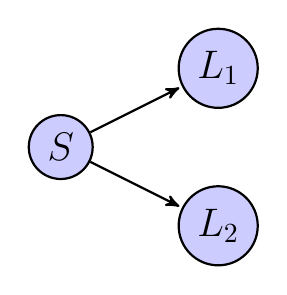
\begin{tikzpicture}[->,>=stealth',shorten >=1pt,auto,node distance=3cm,
  thick,main node/.style={circle,fill=blue!20,draw,
  font=\sffamily\Large\bfseries,minimum size=8mm}]

  \node[main node] (S) at (0,0) {$S$};
  \node[main node] (L1) at (2,1) {$L_1$};
  \node[main node] (L2) at (2,-1) {$L_2$};

  \path[every node/.style={font=\sffamily\small,
          fill=white,inner sep=1pt}]
    (S)  edge (L1)
         edge (L2);

\end{tikzpicture}
\label{fig:exa-trans}
\caption{Simple message passing system}
\end{figure}

Intuitively, there are subsets of the overall state space which are important to understanding the evolution of such a system. For example, let $A_1$ denote the subset of states in which the processor $S$ has not sent a message, let $A_2$ be the subset in which $S$ has broadcast a message, and let $A_3$ be the subset in which $L_1$ and $L_2$ have each received and processed the message. The union $A_1 \cup A_2 \cup A_3$ covers the set of reachable states of the system and defines an ASM that is useful for reasoning about its dynamics and understanding counter-example traces.
\end{example}


% ------------------------------------------------------------

% ------------------------------------------------------------
\section{Putting it Together: Compositional Modeling and Verification for Oral Messages}\label{sec:byz}

To demonstrate the model and techniques, we model an implementation of the Oral Messages Hybrid (OMH) algorithm~\cite{}, a more sophisticated version of the class Oral Messages (OM) algorithm. OM was first formulated by Lamport, Shostak, and Pease~\cite{om} to achieve agreement in a distributed system while tolerating Byzantine faults. OMH was originally developed by Thambidurai and Park~\cite{hybrid} to achieve the same result in the presence of a more sophisticated fault model that includes symmetric and benign faults. However, OMH had a bug, as originally formulated, which was corrected and formally verified by Lincoln and Rushby using interactive theorem-proving~\cite{csl-93-2}.

First, we briefly describe the algorithm, sketch our model of the algorithm within the model presented in Section~\ref{sec:model}, then describe it's invariants.

\subsection{OMH(1) Algorithm}
OMH is a recursive algorithm that proceeds in rounds of communication. Let $OMH(m)$ be a recursive function implementing the algorithm, parameterized by the number of rounds, $m$. Consider a finite set of nodes $N$. Distinguish one node as the \emph{general}, $g$, and the remaining nodes $L = N \setminus \{g\}$ as the \emph{lieutenants}. We assume the identity of any general or lieutenant cannot be spoofed. Broadcast communication proceeds in rounds. Denote any message that is detectably faulty (e.g., fails a CRC) or is absent, by $ERR$. Additionally, in the algorithm, nodes report on values they have previously received. In doing so, nodes must differentiate \emph{reporting} $ERR$ from an $ERR$ itself. Let $R$ denote that an error is being reported. Finally, let $V$ be a special, designated value.

%% The goal of the algorithm is for each of the lieutenants to agree on the value sent by $g$ in the presence of a Byzantine faulty general or lieutenants. More precisely, we assume the identity of a sender cannot be spoofed, broadcast communication proceeds in synchronous rounds such that the absence of a message in a round can be detected by the receiver (let $None$ be a constant used when a message is detectably incorrect, including a lack of message), and a Byzantine faulty sender can arbitrary corrupt or not send a message, but there are no other faults in the system.

The algorithm is recursively defined:

\begin{itemize}
\item {\bf $OM(0)$}: $g$ broadcasts a value to each lieutenant, and the lieutenants return the value received (or $ERR$).
\item {\bf $OM(m)$, $m > 0$}:
  \begin{enumerate}
  \item $g$ broadcasts a value to each lieutenant, $l$.
  \item\label{om:two} Let $l_v$ be the value received by $l \in L$ from $g$. Then for each $l$, execute $OMH(m-1)$, assigning $l$ to be the general and $L \setminus \{l\}$ to be the lieutenants. $l$ sends $l_v$ or $R$, if $l_v = ERR$.
  \item For each lieutenant $l \in L$, remove all $ERR$ values received in Step~\ref{om:two} from executing $OHM(m-1)$. Compute the majority value over the remaining values, or $V$ if there is no majority. If the majority value is $R$, return $E$.
  \end{enumerate}
\end{itemize}

\noindent
In particular, $OMH(1)$ includes two rounds of broadcast communication, one in which the general broadcasts, and one in which the lieutenants exchange their values.

OMH is designed to preserve \emph{validity} and \emph{agreement}
properties. Validity states that if the general is nonfaulty, then every lieutenant outputs the value sent by the general. More formally, let the general broadcast $v \neq ERR$, and let $l_i$ denote the output for lieutenant $i$:
%
\begin{equation}
  \tag{Validity}
    \forall \,i. \quad l_i = v
\end{equation}
%
Agreement states that each lieutenant outputs the same value. Let $l_i, l_j$ denote the outputs of lieutenants $i, j \in L$, respectively:
%
\begin{equation}
  \tag{Agreement}
    \forall \,i, j. \quad l_i = l_j
\end{equation}
%

We described a hybrid fault model in Section~\ref{sec:kibitzer}. Under that fault model, agreement and validity hold if $2a+2s+b+1 \geq n$, where $n$ is the total number of nodes, $a$ is the number of Byzantine (or asymmetric) faults, $s$ is the number of symmetric faults, and $b$ is the number of benign faults. Additionally, it is required that the number of rounds $m$ be greater or equal to the number of Byzantine faults, $a$~\cite{csl-93-2,hybrid}.

\subsection{Model Sketch}
The verification is carried out in the Symbolic Analysis Laboratory~\cite{}, which contains a suite of model-checkers and a high-level specification language. In our work, we use infinite-state (SMT-based) $k$-induction~\cite{}.

\lee{Maybe talk about MJRTY here. Maybe also talk about relaxing in synchronous communication in model.}
\lee{talk about synchrony being loosened, so the general/receivers don't all send/receive at the same time. Talk about lieutenants being ``unrolled'' into relays and receivers, following Rushby.}

\subsection{Invariants}\label{sec:invariants}

%% Lemmas and dependencies:
%% cal:
%%   cal_invt (-)

%% ASM:
%%   abstract_all (cal_invt, receiver_mode_invt)

%% faults:
%%   manifest_relay (-)
%%   uninterp_msg_relay (-)
%%   fault_propagation (cal_invt)
%%   source_to_latch (fault_propagation)
%%   manifest_source (fault_propagation)

%% receiver:
%%   missing_buffer_size (cal_invt)
%%   receiver_mode_invt (missing_buffer_size)

%% voting:
%%   majority_vote_invt (receiver_mode_invt)
%%   exists_majority (receiver_mode_invt majority_vote_invt)

%% protocol: (everything :))
%%   validity
%%   agreement

\begin{figure}
  \centering
  \footnotesize
  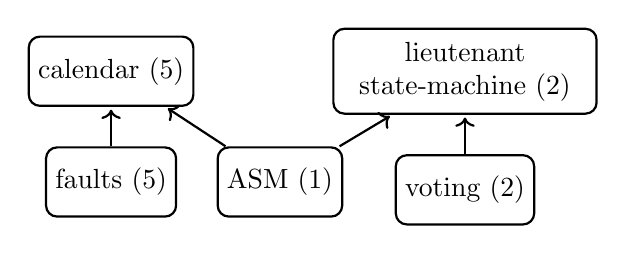
\begin{tikzpicture}[->, node distance=2.6cm, auto, shorten >=1pt, bend angle=45,thick]
    \tikzstyle{every state}=[rectangle, rounded corners]

    \node[state] (calendar) {calendar (5)};
    \node[state] (lieutenant) [right=1.75cm of calendar] {\begin{tabular}{c}lieutenant\\state-machine (2)\end{tabular}};
    \node[state] (faults) [below=0.5cm of calendar] {faults (5)};
    \node[state] (asm) [right=0.5cm of faults] {ASM (1)};
    \node[state] (voting) [below=0.5cm of lieutenant] {voting (2)};

    \tikzstyle{every node}=[]

    \path
    (faults) edge [] node {} (calendar)
    (asm)    edge [] node {} (calendar)
    (asm)    edge [] node {} (lieutenant)
    (voting) edge [] node {} (lieutenant);

  \end{tikzpicture}
  \caption{Invariant classification and dependencies.}
  \label{fig:proof}
\end{figure}

To make the proof scalable, we specify inductive invariants to be used by SAL's $k$-induction engine. There are 11 invariants, falling into five categories:
\begin{enumerate}
  \item \emph{Calendar automata}: Lemmas relating to the calendar automata model. These include lemmas such as time being monotonic, channels missing messages if there is no calendar event, and only nodes associated with a calendar event may execute their local state machines.
  \item \emph{Abstract state machine (ASM)}: Lemmas relating the ASM synchronous observer states to the implementation states.
  \item \emph{Lieutenant local state-machine (SM) behavior}: Lemmas describing the modes of behavior of the lieutenants. The major modes of the state machine are receiving messages, then once it has filled its buffer, it votes, and after voting returns the result. One additional lemma notes that the messages currently received plus missing messages equals the total number of expected messages.
  \item \emph{Faults}: Lemmas characterizing the effect of a fault in a single broadcast. Examples include lemmas stating that if a node receives a faulty message, some ``upstream'' node in the communication path was faulty. Another example is that the faults of messages latched by a node in its buffer match the faults ascribed to the sender in the calendar event.
  \item \emph{Voting}: Lemmas proving that the Fast Majority Vote algorithm implements a majority vote, if one exists. These lemmas are nearly verbatim transcriptions from the journal proofs~\cite{mjrty}.
\end{enumerate}
\noindent
The proof structure is shown in Figure~\ref{fig:proof}. The number of lemmas per category are shown in parentheses. Arrows denote dependencies. For example, the ASM lemmas depend on both the calendar automata and lieutenant state-machine lemmas. As can be seen, the proof structure is quite modular. The calendar lemmas are general and independent of any particular protocol or fault model. Similarly, lemmas about the internal behavior of a lieutenant is independent of the global protocol behavior. It is also independent of the effect of faults on the system---the only ``knowledge'' of faults that lieutenant has is whether a fault is benign or not. Lemmas about the behavior of faults in the system are also independent of the particular protocol being modeled. Likewise, lemmas about the particular voting algorithm used depend only on the lieutenant's internal behavior. Only the ASM depends on both calendar-specific and local state-machine results, since it is an abstraction of the entire system implementation. Recall, however, that the ASM is a convenience for debugging and can be elided.

% ------------------------------------------------------------
\section{Experimental Results}\label{sec:experimental}

Here we present two classes of experimental results. First, we demonstrate the scalability results of the verification, despite the low-level modeling. Then we describe modularity results, demonstrated by making modifications to the model and re-validating the model.

\subsection{Scalability}

\begin{figure}
  \centering
  \begin{tabular}{r||c|c|c|c|c|c|c|c|c|c|}
      \multicolumn{11}{c}{Receivers} \\
      \cline{2-11}
   Relays &   1  &  2  &   3  &  4  &   5  &  6   &  7   &  8  &  9  &  10 \\
      \hline \hline
      1   & 7    & 9   & 12   & 15  & 21   & 25   & 32   & 40  & 54  & 74  \\
      \hline
      2   & 17   & 14  & 21   & 30  & 42   & 53   & 74   & 99  & 144 & -   \\
      \hline
      3   & 21   & 22  & 40   & 50  & 81   & 102  & 155  & 279 & -   & -   \\
      \hline
      4   & 27   & 34  & 59   & 99  & 141  & 237  & 1114 & -   & -   & -   \\
      \hline
      5   & 22   & 94  & 125  & 335 & TO   & 1406 & -    & -   & -   & -   \\
      \hline
      6   & 36   & 132 & 2966 & 844 & 2457 & -    & -    & -   & -   & -   \\
      \hline
      7   & 83   & 487 & TO   & TO  & -    & -    & -    & -   & -   & -   \\
      \hline
      8   & 298  & TO  & TO   & -   & -    & -    & -    & -   & -   & -   \\
      \hline
      9   & 1428 & TO  & -    & -   & -    & -    & -    & -   & -   & -   \\
      \hline
     10   & TO   & -   & -    & -   & -    & -    & -    & -   & -   & -   \\
      \hline
  \end{tabular}
  \label{fig:benchmark}
  \caption{Benchmark of full proof computation time for OMH(1) implementation. Times are in seconds with a timeout (TO) limit of one hour. Dashes ('-') denote no benchmark was run.}
\end{figure}

The benchmarks were performed on a server with Intel Xeon E312xx (Sandy
Bridge) CPUs (mid 2011).

For comparison, when the fault model is ``turned off'' by defining the fault
type to contain a single 'nonfaulty' value and removing fault specific lemmas,
model-checking scales further. For example when there are 3 relays and 3
receivers the time is 25s (compared to 40s above), and when where are 5 relays
and 5 receivers the time is 315s (compared to timeout above). See Figure
\ref{fig:effort} for more comparisons.

\lee{discuss results}

\subsection{Modular Verification}\label{sec:modular}

\begin{figure}
  \centering
  \begin{tabular}{p{3cm}|p{3cm}|l|l|}
                                  & Modules modified    & Lemmas modified & Lemma classes modified\\
  \hline \hline
  Byzantine-only fault model      & 0                   & 0               & 0 \\
  \hline
  Time-triggered message-passing  & \texttt{clock}, \texttt{relay}
                                  , \texttt{receiver}   & 0               & 0 \\
  \hline
  \end{tabular}
  \caption{Refactoring effort for protocol modifications.}
  \label{fig:effort}
\end{figure}
To demonstrate the modularity of the model and verification approach, in this section, we explore variants to the model and discover the effort required to implement the modifications and repair the proofs. The results are summarized in Figure~\ref{sec:effort} and sketched below.

\paragraph{Fault model.}
Modifying the fault model is easy. In involves modifying the definition of a single function, \texttt{mfa}, that takes as an argument the static assignment of node identifiers to faults. Moreover

\paragraph{Time-triggered messaging.}

\subsection{Proof Effort Remarks}
The lemmas described in Section~\ref{sec:invariants} are constructed by-hand and represent multiple days of effort, but that effort includes both model and protocol construction and generalization as well as verification. The counterexamples returned by SAL are very useful for strengthening invariants, but tedious to analyze---a model with five relays and two receivers contains 90 state variables, and there are known counterexamples to models that size~\cite{csl-93-2}. Once we developed the ASM synchronously-composed observer, the verification effort was sped up considerably.

As shown in Section~\ref{sec:modular}, modifications to the implementation are modular. In particular, any protocol specified in the model can reuse the lemmas associated with the calendar automata and fault-model (insofar as they use the same fault model).

Moreover, we are agnostic about how lemmas are discovered. As techniques like IC3 scale, they may be discovered automatically. $k$-induction in infinite-state model-checking blurs the lines between interactive and automated theorem proving. IC3 can even be strengthened using $k$-induciton~\ref{pdr-kind}. Tools like Ivy can present graphical counterexamples to help interactively develop invariants~\cite{ivy}.

% ------------------------------------------------------------
\section{Related Work}\label{sec:related}

The Oral Messages algorithm and its variants have a long history of formal verification, making it a good test-case for comparing and contrasting verification tools~\cite{pvs}. The Oral Messages algorithm was presented in the landmark paper by Lamport, Shostak, and Pease~\cite{om}. Later, a hybrid fault-model and modified Oral Messages algorithm was developed by Thambidurai and Park~\cite{hybrid}. OM(1) was subsequently verified in both the PVS and ACL2 interactive theorem-provers~\cite{Young97:IC}. Also in ACL2, an implementation of a circuit design to implement OM(1) is given~\cite{om-acl2-impl}; the low-level model most closely relates to our level of detail. A refinement-based verification approach is used, and OM(1) is specialized to a four-process system. Using the PVS interactive theorem-prover~\cite{pvs}, Lincoln and Rushby demonstrate a flaw in Thambidurai and Park's algorithm and present a fix to it~\cite{csl-93-2}.

Using automated techniques, Gasc{\'{o}}n and Tiwari use SAT-based bounded synthesis to partially synthesize a variant of Oral Messages that tolerates transient faults~\cite{om1-synth}. Bokor~\emph{et~al.} describe a message-passing model for synchronous distributed algorithms that is particularly amenable to partial-order reduction for explicit-state model-checking~\cite{Bokor2010}. That said, their model of OM(1) (not OMH(1)), timeouts after 10~hours, and we assume a voting algorithm is not explicitly specified. \lee{for what size? Also, Rushby's model?} Very recently, Jovanovi{\'{c}} and Dutertre use a ``flattened'' high-level model of OM(1) as a benchmark for IC3 augmented with $k$-induction~\cite{pdr-kind}.

\lee{mention that ASMs similar to disjunction invariants}

% ------------------------------------------------------------
\section{Conclusions}\label{sec:conclusions}
This work fits within a larger project, in collaboration with Honeywell Labs, to build an \emph{architectural domain-specific language} (ADSL) for specifying and verifying distributed fault-tolerant systems. The goal of the language is to synthesize both software and/or hardware implementations as well as formal models for verification. Before building such an ADSL, we needed a scalable general formal model to which to compile, leading to the work presented. An ADSL will make refactoring even easier. We have developed a preliminary ADSL that generates C code as well as formal models SRI's Sally~\cite{}, a model-checking descendent to SAL that will be described in a subsequent paper.\footnote{\url{https://github.com/GaloisInc/atom-sally}}

\lee{link to all results in github}
\lee{talk about compositional verification of properties, even though SAL doesn't directly support it}
\lee{talk about k-induction vs. PDR}
\lee{talk about lack of axiomatization in model-checking (multiple rushby bugs), but  tradeoff of deadlock. see proglema paper}
\lee{note some details still elided for implementation ---e.g., CRCs, etc.}

\section*{Acknowledgments}
This work is partially supported by NASA contract \#NNL14AA08C. We are indebted to our collaborators Brendan Hall and Srivatsan Varadarajan at Honeywell Labs, and to Wilfredo Torres-Pomales at NASA Langley for their discussions and insights.

\bibliographystyle{IEEEtran}
\bibliography{paper}

\end{document}
